\documentclass{article}

\usepackage{xeCJK}
\usepackage{graphicx}
\usepackage{caption}
\usepackage{subfigure}
\usepackage[colorlinks=true,
linkcolor=blue
]{hyperref}
\usepackage{listings}
\usepackage[outputdir=build]{minted}
\usepackage{amsmath}
\usepackage{lastpage}   %获得总页数
\usepackage{fancyhdr}
\usepackage{bookmark}
\graphicspath{{../img/}}
\pagestyle{fancy}
\setlength{\headheight}{64pt}
\lhead{}
\chead{}
\rhead{}
\lfoot{}
\cfoot{}
\rfoot{\thepage\ of \pageref{LastPage}} % 当前页 of 总页数
\renewcommand{\headrulewidth}{0.4pt}    % 改为0pt即可去掉页眉下面的横线
\renewcommand{\footrulewidth}{0.4pt}    % 改为0pt即可去掉页脚上面的横线
\lhead{
\includegraphics[height=0.8in]{depsast.jpg}}  % 插入科协LOGO
\setCJKfamilyfont{yy}{YouYuan}                       % 幼圆  yy

\newcommand{\yy}{\CJKfamily{yy}}
\renewcommand{\baselinestretch}{1.6}

\makeatletter
\renewcommand\paragraph{\@startsection{paragraph}{4}{\z@}%
            {-2.5ex\@plus -1ex \@minus -.25ex}%
            {1.25ex \@plus .25ex}%
            {\normalfont\normalsize\bfseries}}  % make paragraph act like 'subsubsubsection'
\makeatother
\setcounter{secnumdepth}{4} % how many sectioning levels to assign numbers to
\setcounter{tocdepth}{4}    % how many sectioning levels to show in ToC

\graphicspath{{./img/ccd/}{./img/}}

\begin{document}


\title{6-6 线性CCD模块介绍}
\author{工程物理系学生科协技术部\quad 高一川}
\date{\today}
\maketitle
\tableofcontents
\newpage


\section{前言}
线性 CCD 模块是智能车的“眼睛”,本文档旨在向大家阐述线性 CCD 的基本原理及其软硬件使用说明。

\section{线性 CCD 简介}

\subsection{与面阵 CCD 的区别}

说到 CCD,想必大家都不陌生。在我们常用的手机、数码相机等电子设备的摄像头中,CCD 得到了广泛的应用。但是细心的各位可能发现了,我们这篇文档从始至终都在强调“线性” CCD,那么什么是线性 CCD,它又与我们常说的 CCD 有什么区别呢?

我们常说的 CCD 指的是面阵 CCD,在你使用手机拍照后,会得到一幅图像,如果你感兴趣的话,打开图像的属性可以看到它的尺寸,例如 1920x1080。从此可以发现,手机里面的 CCD 拍下的图像可以被认为是一个 1920x1080 的矩阵(这里只考虑灰度图像)。但是如果你使用线性 CCD 拍摄下同样一幅图像,你会发现它的尺寸是 1x128,也就是说线性 CCD 拍下的图像是一个仅有一个像素宽的长条,我们可以将其作为一个由 128 个灰度值组成的向量(数组),这也就是两种 CCD 最大的不同之处。两种 CCD 拍到的图片如下图所示。

\begin{figure}[h]
 \centering
 \captionsetup{labelformat=empty}
 \begin{minipage}[t]{0.35\textwidth}
  \centering
  
\includegraphics[width=\linewidth]{common_ccd.jpg}
  \caption{\scriptsize{面阵 CCD 拍到的赛道图像}}
 \end{minipage}
 \begin{minipage}[t]{0.35\textwidth}
  \centering
  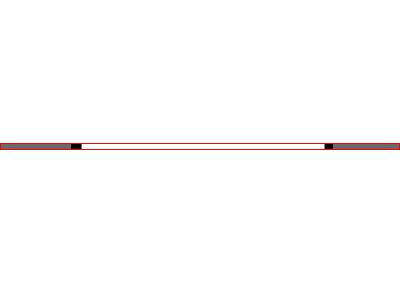
\includegraphics[width=\linewidth]{linear_ccd.jpg}
  \caption{\scriptsize{线性 CCD 拍到的赛道图像}}
 \end{minipage}
\end{figure}

\subsection{模块引脚介绍}

本届智能车大赛提供的线性 CCD 模块的主芯片为 TSL1401CL 芯片,模块共引出了六个引脚,各引脚的功能及其与单片机 IO 口的连接如下表:

\begin{table}[]
 \centering
 \captionsetup{labelformat=empty}
 \caption{线性 CCD 模块引脚功能}
 \label{ccd_pinouts}
 \begin{tabular}{|l|l|l|l|}
  \hline
  引脚序号 & 名称 & 连接的 IO 口 & 功能描述    \\ \hline
  1            & GND    & GND              & 地线          \\
  2            & VDD    & 3V3              & 3.3V 电源     \\
  3            & AO     &                  & 模拟量输出 \\
  4            & CLK    &                  & 时钟输入    \\
  5            & SI     &                  & 串行输入    \\
  6            & AM     & NC               & 无连接       \\ \hline
 \end{tabular}
\end{table}

\subsection{功能及时序描述}

TSL1401 芯片包含 128 个线性排列的光电二极管,同时片内为每个光电二极管集成了独自的积分电路,下面为了便于理解,我们将这些光电二极管及其积分电路统称为像素。对于每个像素来说,其采集到的灰度值均与其感知的光强与积分(曝光)时间成正比,而采集到的灰度值将在 AO 线上以模拟信号(电压)的形式输出,下面将每个像素采集到的灰度值称为其像素值。那么问题来了,我们共有 128 个像素值要传输给单片机,但是 AO 线只有一根,怎么办呢?这时候就轮到 CLK 和 SI 这两个信号上场了。

如果你去查阅 TSL1401 芯片的数据手册,你会看到如图的时序图


\end{document}
